\documentclass[12pt,a4paper]{article}

% === PAQUETES === (((
\usepackage{amsmath}
\usepackage{colortbl}
\usepackage{amsfonts}
\usepackage{multicol}
\usepackage{multirow}
\usepackage{xcolor}
\usepackage{amssymb}
\usepackage{listings} 
% \usepackage{expl3}
\usepackage{fontspec}
\usepackage{fullpage}
\usepackage{graphicx}
\usepackage{titlesec} 
% \usepackage{setspace}
\usepackage{dsfont}
% \usepackage{bookmark}
% )))

% === TIPOGRAFÍA === (((
\setmainfont[
  BoldFont       = bodonibi,
	ItalicFont     = Century modern italic2.ttf,
	BoldItalicFont = bodonibi,
	SmallCapsFont  = lmromancaps10-regular.otf
]{Century_modern.ttf}
% )))

% === COMANDOS === (((
\newcommand{\dis}{\displaystyle}
\newcommand{\qed}{\hspace{0.5cm}\rule{0.16cm}{0.4cm}}
\newcommand{\micita}[1]{\([\)\cite{#1}\(]\)}
\newcommand{\operator}[1]{\mathop{\vphantom{\sum}\mathchoice{ \vcenter{\hbox{\huge $#1$}} }
{\vcenter{ \hbox{\Large $#1$}} }{#1}{#1}}\displaylimits}
\newcommand{\suma}{\operator{ \includegraphics[scale=0.09]{IMAGENES/Sigma.png}} }
\DeclareSymbolFont{italics}{\encodingdefault}{\rmdefault}{m}{it}
\DeclareSymbolFontAlphabet{\mathit}{italics}
\ExplSyntaxOn
\int_step_inline:nnnn { `A } { 1 } { `Z }
 {  \exp_args:Nf \DeclareMathSymbol{\char_generate:nn{#1}{11}}{\mathalpha}{italics}{#1} }
\int_step_inline:nnnn { `a } { 1 } { `z } {  \exp_args:Nf \DeclareMathSymbol{\char_generate:nn{#1}{11}}{\mathalpha}{italics}{#1}}
\ExplSyntaxOff
% )))

% === SECCIONES === (((
\titleformat*{\section}{\large\normalfont\bfseries}
\titleformat*{\subsection}{\large\itshape}
\titleformat*{\subsubsection}{\bfseries\centering}
% \setcounter{secnumdepth}{0}
\renewcommand*{\contentsname}{\large\textbf{CONTENIDOS.}}
\usepackage[nottoc,numbib]{tocbibind}
\renewcommand{\refname}{REFERENCIAS.}
\renewcommand{\tablename}{Tabla}
\renewcommand{\figurename}{Figura}
% )))

% === PORTADA === (((
% \pagestyle{empty}
\newcommand{\portada}{
\addfontfeature{LetterSpace=-5}
  \begin{titlepage}
  \centering
  \begin{figure}
    \centering
    \includegraphics[scale=0.5]{IMAGENES/logo_uaa.png}  
  \end{figure}
  {\bfseries\Large\MakeUppercase{\textit{Universidad Autónoma de Aguascalientes.}} \par}
  \vspace{1cm}
  {\Large Centro de Ciencias Básicas. \vspace{0.5cm}\\[2mm]
  Departamento de Matemáticas y Física.\vspace{0.5cm}\\[2mm]
  Licenciatura en Matemáticas Aplicadas.\vspace{0.5cm}\\[2mm]
  Práctica 7.\par}
  \vspace{1.5cm}
  {\bfseries\Huge Difracción. \par} % title
  \vspace{1.5cm}
  {\itshape\Large Óptica. \\Prof. Mariana Alfaro Gómez.\par}
  % {\itshape\Large Variable Compleja I. \\Prof. Fausto Arturo Contreras Rosales.\par}
  % {\itshape\Large Métodos Numéricos II. \\Prof. Manuel Ramírez Aranda.\par}
  % {\itshape\Large Diseño de Experimentos. \\Prof. Angélica Hernández Quintero.\par}
  % {\itshape\Large Filosofía de la Investigación Científica. \\Prof. Jesús Mariano Rodríguez Muñoz.\par}
  \vfill
  % {\Large \textit{Por Erick I. Rodríguez Juárez.}\par}
		\begin{flushleft}
		\Large
		Alumnos:\\
		\textit{Carlos Francisco Guzmán Barba.}\\
		\textit{Erick Ignacio Rodríguez Juárez.}\\
		\textit{Manuel Alejandro Siller Landin.}
		\end{flushleft}
	% {}  % {\Large \textit{Por Erick I. Rodríguez Juárez.}\par}
  \vfill
		\begin{flushright}
		{\Large Realización: 16\(/\)05\(/\)22. \par} % date
		{\Large Entrega: 23\(/\)05\(/\)22. \par} % date
		\end{flushright}
  \end{titlepage} 
	% \thispagestyle{empty}
	% \doublespacing
	% \tableofcontents
	% \singlespacing
	% \newpage
} 
% )))

% === LST-LISTINGS PARA VER EL CÓDIGO === (((
\usepackage{xcolor}
\definecolor{backcolour}{rgb}{0.95,0.95,0.92}

\lstdefinestyle{mystyle}{
  backgroundcolor  =  \color{backcolour},
  commentstyle     =  \color{gray},
  numberstyle      =  \tiny\color{gray},
  stringstyle      =  \color{purple},
  basicstyle       =  \ttfamily\footnotesize,
  numbers          =  left,
  numbersep        =  5pt,
  keywordstyle     =  \color{blue},
  identifierstyle  =  \color{orange},
}

\lstset{style=mystyle}
% )))

\begin{document}

\portada

\section{RESUMEN.} % (((
% )))

\section{INTRODUCCIÓN.} % (((

\subsection{--- Marco Teórico ---} % (((
\label{sub:marco_teorico}
Consideremos el siguiente sistema físico. En la Figura \ref{fig:constructiva} (obtenida de \micita{serway}) se tiene el experimento de Young, que consiste en la transmisión de una única onda a través de dos ranuras (\(S_1\) y \(S_2\)) colocadas en una pared contra la que choca la onda.
Además, se registra el patrón de ondas generado en una segunda pared ubicada a una distancia \(L\) de la primera (cuyo centro está en \(O\)), y haremos el análisis para un punto \(P\) en ella.
Sea \(d\) la distancia de separación entre las rejillas, y supondremos que \(d \ll L\).
Debido a ésto, \(S_2R \approx r_2-r_1\), y además \(QP \perp S_1R\), por lo que el ángulo \(\angle S_2S_1R \approx \angle OQP = \theta\), el \textit{ángulo de desviación} de la onda.
\begin{figure}[hbtp!]
	\addfontfeature{LetterSpace = -5}
	\centering
	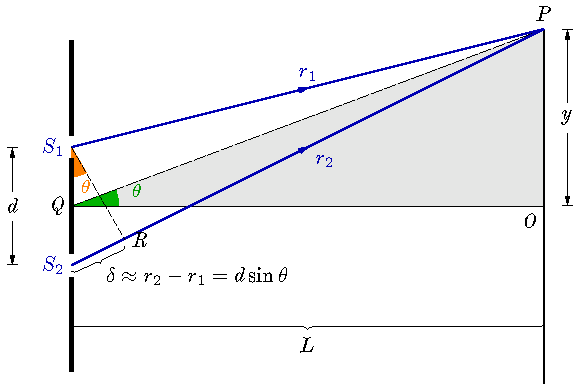
\includegraphics[width= 0.8 \linewidth]{1_INTRO/1/tikz.pdf}
	\caption{Experimento de la Doble Rendija de Young.}
	\label{fig:constructiva}
\end{figure}\\
Notamos que la interferencia total que se obtendrá en el punto \(P\), queda completamente determinada por la diferencia de longitudes \(r_2-r_1\), puesto que en cualquier trayecto de longitud \(r_1\), la onda se comporta de la misma manera.
La interferencia es constructiva siempre que \(r_1-r_2 = m \lambda\), para algún \(m \in \mathds{Z}\). Es decir
\begin{equation}
	d \sin \theta = m \lambda , \hspace{1cm} m \in \mathds{Z} .
	\label{eq:young}
\end{equation}
donde se alcanzará un máximo cuando \(m \in \mathds{Z}\). Y si \(m=k/2\), con \(k\) impar, entonces se alcanzará un mínimo. Además, el campo eléctrico \(E_i\) en el punto \(S_i\) está dado por
\begin{equation}
	\begin{array}{rcl}
		E_1 & = & E_0 \sin wt \\[2mm]
		E_2 & = & E_0 \sin (wt+ \phi)
	\end{array}
	\label{eq:campos_electricos}
\end{equation}
Y por el principio de superposición, tendremos que el campo eléctrico total es:
\begin{equation}
	E = E_1 + E_2 = (2E_0 \cos \beta) \sin (wt+ \beta).
	\label{eq:campo_total}
\end{equation}
donde \(\beta = \phi /2\). Recordamos que \(\beta = \dfrac{2 \pi \sin \theta}{\lambda}\), y la intensidad para el ángulo \(\theta\) está dada por
\begin{equation}
	I(\theta) = 4I_0 \cos ^2 \beta = 4I_0 \cos ^2 \bigg(\dfrac{\pi d \sin \theta}{\lambda}\bigg).
	\label{eq:intensidad}
\end{equation}
Los máximos son alcnazados cuando
\begin{equation}
	W \sin \theta = n \lambda , \hspace{1cm} n \in \mathds{Z}
	\label{eq:maximos}
\end{equation}
y análogamente al caso anterior, se tiene que
\begin{equation}
	\theta = \arctan (y/L).
	\label{eq:theta}
\end{equation}
Consulte la teoría en \micita{alonso_finn_1}.
% )))

\subsection{--- Análisis Experimental ---} % (((
\label{sub:analisis_experimental}
El propósito de el sistema experimental es el de presenciar el patrón de difracción y el patrón de interferencia en el sistema de la doble rendija.
Además, de observar el cambio producido en el fenómeno por diferentes longitudes de onda dentro del rango humano visible.
Por tanto, para rejillas proporcionales a la longitud de onda, se espera que el patrón de difracción, cree el patrón de onda para la longitud de onda correspondiente.
En consecuencia, para una sola longitud de onda se tendrá el patroń de la Figura \ref{fig:una_lon}. Y para varias longitudes de onda, se tendrá el patrón de la Figura \ref{fig:var_lon}, cuando todas las longitudes de onda del espectro visible impacten la rejilla.
\begin{figure}[hbtp!]
	\addfontfeature{LetterSpace = -5}
	\begin{minipage}{0.5\linewidth}
		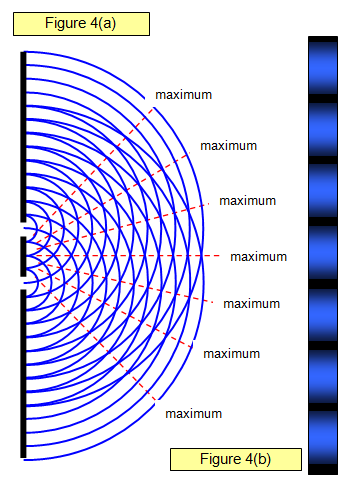
\includegraphics[width= 0.7 \linewidth]{1_INTRO/4}
		\caption{Patrón de onda para una sóla longitud de onda.}
		\label{fig:una_lon}
	\end{minipage}\hspace{5mm}
	\begin{minipage}{0.5\linewidth}
		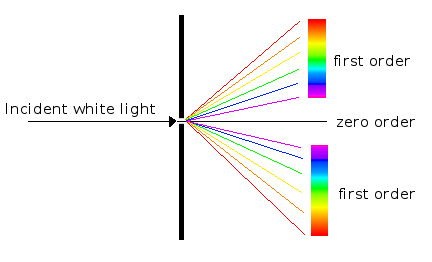
\includegraphics[width= \linewidth]{1_INTRO/5}
		\caption{Patrón de onda para las longitudes de onda del espectro humano visible.}
		\label{fig:var_lon}
	\end{minipage}
\end{figure}
% )))

% )))

\section{METODOLOGÍA.} % (((
La incertidumbre de la regla y la cinta métrica empleados era de $ \dfrac{0.1 cm}{2}=0.05 cm $
\subsection{--- Difracción de una Rendija Simple y Doble Rendija ---} % (((
\label{sub:difraccion_simple}

\subsubsection{Rendija Simple.} % (((
\label{subs:rendija_simple}
% )))

\subsubsection{Doble Rendija.} % (((
\label{subs:doble_rendija}
% )))

% )))

\subsection{--- Rejilla de Difracción. ---} % (((
\label{sub:reijlla_de_difraccion}
% )))

% )))

\section{RESULTADOS.} % (((

\subsection{--- Difracción de una Rendija Simple y Doble Rendija ---} % (((
\label{sub:resul_difraccion_simple}
Para la primera parte del experimento, donde se emplearon los filtros de colores, se obtuvieron las siguientes mediciones mostradas en la tabla \ref{tab:1}.
\begin{table}[!htb]
\centering
\caption{Difracción en una rendija simple.}
\begin{tabular}{|c|c|c|c|c|}
	\hline
	Color & $ n $ & $ W $ (mm) & $ y\mbox{ }(\pm0.05\mbox{ cm})$  & L $(\pm0.05\mbox{ cm})$ \\	\hline
	\rowcolor{red!25}
	\cellcolor{red!40}{Rojo} & 2 & 0.04 & 1.25 & 25 \\	\hline
	\rowcolor{green!25}
	\cellcolor{green!40}{Verde} & 2 & 0.04 & 1 & 25 \\	\hline
	\rowcolor{blue!25}
	\cellcolor{blue!40}{Azul} & 2 & 0.04 & 0.9 & 25 \\	\hline
\end{tabular}
\label{tab:1}
\end{table}\\
Entonces, en la tabla \ref{tab:2} se encuentran los resultados para la estimación de la longitud de onda de la luz empleada.
\begin{table}[!htb]
\centering
\caption{Estimación de $ \lambda $.}
\begin{tabular}{|c|c|c|}
	\hline
	Color & $ \theta $ (rad) & $ \lambda $ (nm)\\	\hline
	\rowcolor{red!25}
	\cellcolor{red!40}{Rojo} & $ 0.0499\pm 0.0020 $ & $ 998.7523\pm 41.8429 $ \\	\hline
	\rowcolor{green!25}
	\cellcolor{green!40}{Verde} & $ 0.0399\pm 0.0020 $ & $ 799.3608\pm 41.5003 $ \\	\hline
	\rowcolor{blue!25}
	\cellcolor{blue!40}{Azul} & $ 0.0359\pm 0.0020 $ & $ 719.5339\pm 41.3595 $ \\	\hline
\end{tabular}
\label{tab:2}
\end{table}
% )))

\subsection{--- Rejilla de Difracción. ---} % (((
\label{sub:resul_reijlla_de_difraccion}
Para el segundo experimento, se empleó la rejilla de difracción con 
$$ A=6000\dfrac{aberturas}{cm} $$
separada a una distancia $ L=(25\pm0.05)\mbox{ cm} $ tanto de la fuente como de la retina del ojo.
Se obtuvieron entonces las siguientes mediciones, las cuales se muestran en la tabla \ref{tab:3}.
\begin{table}[!htb]
\centering
\caption{Datos para el cálculo del rango de $ \lambda $.}
\begin{tabular}{|c|c|c|}
	\hline
	Color & $ y_1\mbox{ }(\pm0.05\mbox{ cm})$ & $ y_2\mbox{ }(\pm0.05\mbox{ cm})$ \\ \hline
	\rowcolor{violet!25}
	\cellcolor{violet!40}{Violeta}  & 5.5 & 14   \\ \hline
	\rowcolor{blue!25}
	\cellcolor{blue!40}{Azul}     & 6.5 & 15.5 \\ \hline
	\rowcolor{green!25}
	\cellcolor{green!40}{Verde}    & 7   & 18   \\ \hline
	\rowcolor{yellow!25}
	\cellcolor{yellow!40}{Amarillo} & 8   & 20   \\ \hline
	\rowcolor{orange!25}
	\cellcolor{orange!40}{Anaranjado} & 8.5 & 20.5 \\ \hline
	\rowcolor{red!25}
	\cellcolor{red!40}{Rojo}     & 10  & 23   \\ \hline
\end{tabular}
\label{tab:3}
\end{table}\\
Empleando la fórmula (\ref{eq:theta}), se obtuvieron los siguientes resultados (tabla \ref{tab:4.1}).
\begin{table}[!htb]
\centering
\caption{Resultados de la estimación de $ \lambda $ para cada color.}
\begin{tabular}{|l|c|c|c|}
	\hline
	Color & $ \lambda_1(\mbox{nm})$ & $ \lambda_2(\mbox{nm})$ & Promedio $ \lambda (\mbox{nm}) $ \\
	\hline
	\rowcolor{violet!25}
	\cellcolor{violet!40}{Violeta}  & $ 346.4805\pm3.7237 $ & $ 408.3907\pm1.9001 $ & $ 377.4356\pm2.8119 $ \\ \hline
	\rowcolor{blue!25}
	\cellcolor{blue!40}{Azul}     & $ 406.9889\pm3.7766 $ & $ 443.9966\pm1.8722 $ & $ 425.4927\pm2.8244 $ \\ \hline
	\rowcolor{green!25}
	\cellcolor{green!40}{Verde}    & $ 436.8139\pm3.7982 $ & $ 499.2184\pm1.8124 $ & $ 468.0162\pm2.8053 $ \\ \hline
	\rowcolor{yellow!25}
	\cellcolor{yellow!40}{Amarillo} & $ 495.5247\pm3.8316 $ & $ 539.7928\pm1.7560 $ & $ 517.6587\pm2.7938 $ \\ \hline
	\rowcolor{orange!25}
	\cellcolor{orange!40}{Anaranjado} & $ 524.3816\pm3.8436 $ & $ 549.4541\pm1.7412 $ & $ 536.9179\pm2.7924 $ \\ \hline
	\rowcolor{red!25}
	\cellcolor{red!40}{Rojo}     & $ 608.8102\pm3.8620 $ & $ 595.0045\pm1.6637 $ & $ 601.9073\pm2.7629 $ \\ \hline
\end{tabular}
\label{tab:4.1}
\end{table}\\
Los rangos para la longitud de onda de los colores se muestran en la tabla \ref{tab:5.1}.
\begin{table}[!htb]
\centering
\caption{Rangos para $ \lambda $ de cada color.}
\begin{tabular}{|l|c|}
	\hline
	Color & $ \lambda(\mbox{nm})$ \\
	\hline
	\cellcolor{violet!40     }{Violeta   } & \cellcolor{violet!25     }{$ 400 - 455 $}  \\ \hline
	\cellcolor{blue!40       }{Azul      } & \cellcolor{blue!25       }{$ 455 - 490 $}  \\ \hline
	\cellcolor{green!40!white}{Verde     } & \cellcolor{green!25!white}{$ 490 - 570 $}  \\ \hline
	\cellcolor{yellow!40     }{Amarillo  } & \cellcolor{yellow!25     }{$ 570 - 590 $}  \\ \hline
	\cellcolor{orange!40     }{Anaranjado} & \cellcolor{orange!25     }{$ 590 - 620 $}  \\ \hline
	\cellcolor{red!40        }{Rojo      } & \cellcolor{red!25        }{$ 620 - 780 $}  \\ \hline
\end{tabular}
\label{tab:5.1}
\end{table}\\
Y a partir de estos valores, se obtuvieron los siguientes errores absolutos (calculados entre el valor promedio de $ \lambda $ y el mínimo valor de cada rango) mostrados en la tabla \ref{tab:6.1}.
\begin{table}[!htb]
\centering
\caption{Cálculo del error absoluto para $ \lambda $}
\begin{tabular}{|l|c|}
	\hline
	Color & $ |\lambda_{\tiny\mbox{Estimado}}-\lambda_{\tiny\mbox{Tabla \ref{}}}| (\mbox{nm})$ \\
	\hline
	\cellcolor{violet!40     }{Violeta   } & \cellcolor{violet!25     }{$ 22.5644 $}  \\ \hline
	\cellcolor{blue!40       }{Azul      } & \cellcolor{blue!25       }{$ 29.5073 $}  \\ \hline
	\cellcolor{green!40!white}{Verde     } & \cellcolor{green!25!white}{$ 21.9838 $}  \\ \hline
	\cellcolor{yellow!40     }{Amarillo  } & \cellcolor{yellow!25     }{$ 52.3416 $}  \\ \hline
	\cellcolor{orange!40     }{Anaranjado} & \cellcolor{orange!25     }{$ 53.0821 $}  \\ \hline
	\cellcolor{red!40        }{Rojo      } & \cellcolor{red!25        }{$ 18.0927 $}  \\ \hline
\end{tabular}
\label{tab:6.1}
\end{table}
% )))

% )))

\section{DISCUSIÓN DE RESULTADOS Y CONCLUSIONES.} % (((
% )))

% === REFERENCIAS === (((
\bibliography{Referencias}
\bibliographystyle{unsrt}
% )))

\section{APÉNDICE.} % (((

\subsection{--- Propagación de la Incertidumbre ---}
La propagación de la incertidumbre para un producto y un cociente están dadas, respectivamente por
\begin{align*}
(x\pm\delta x)(y\pm\delta y)&=x\cdot y\pm\left(|y|\delta x+|x|\delta y \right)\\\\
\dfrac{x\pm\delta x}{y\pm\delta y}&=\dfrac{x}{y}\pm\left(\dfrac{\delta x}{|y|}+|x|\dfrac{\delta y}{|y|^2}\right)
\end{align*}
Ahora, recordar que si $f$ es una función de $\mathbb{R}^n$ a $\mathbb{R}$ en la cual se le pueden medir sus variables (cada una asociada con su respectiva incertidumbre)
$$f(x_1\pm\Delta x_1,x_2\pm\Delta x_2,...,x_n\pm\Delta x_n)$$
entonces la propagación de la incertidumbre está dada por 
$$\Delta f=\pm\left(\displaystyle\sum_{i=1}^k\Delta x_i\cdot\left|\dfrac{\partial f(x_i)}{\partial x_i}\right| \right)$$
En esta práctica se emplearán las siguientes
\begin{itemize}
\item [$\cdot$] Función $ sen(\theta) $
En este caso
$$f(x\pm\Delta x)=sen(\theta\pm\Delta\theta)\Longrightarrow \Delta f=\Delta\theta\cdot\left|\dfrac{d sen(\theta)}{d\theta}\right|=\Delta\theta\cdot|cos(\theta)|$$
Por lo que 
$$sen(\theta\pm\Delta\theta)=sen(\theta)\pm\Delta\theta\cdot|cos(\theta)|$$
\item [$\cdot$] Función $ arctan(\theta) $
Se tiene que 
$$f(x\pm\Delta x)=arctan(\theta\pm\Delta\theta)\Longrightarrow \Delta f=\Delta\theta\cdot\left|\dfrac{d \mbox{ }arctan(\theta)}{d\theta}\right|=\Delta\theta\cdot\left|\dfrac{1}{\theta^2 + 1 }\right|$$
Y entonces 
$$arctan(\theta\pm\Delta\theta)=arctan(\theta)\pm \dfrac{\Delta\theta}{\theta^2 + 1 }$$
\end{itemize} 

\newpage

\subsection{--- Estimación de la longitud de onda ---}
A partir de los datos de la tabla \ref{tab:1} y empleando lo descrito al inicio del apéndice junto con las fórmulas (\ref{eq:maximos}) y (\ref{eq:theta}), se tiene lo siguiente.
\begin{itemize}
\item [$\cdot$] Filtro Rojo
\begin{align*}
\dfrac{y}{L}=\dfrac{(1.25\pm 0.05)\mbox{ cm}}{(25\pm 0.05)\mbox{ cm}}&=
\dfrac{1.25}{25}\pm\left(\dfrac{0.05}{25}+1.25\cdot\dfrac{0.05}{25^2}\right)=
0.05 \pm 0.0021\\\\
\Longrightarrow arctan(	0.05 \pm 0.0021)&=
arctan(0.05)\pm\dfrac{0.0021}{(0.05)^2+1}=0.0499\pm 0.0020\\\\
\Longrightarrow sen(0.0499\pm 0.0020)&=sen(0.0499)\pm 0.0020\cdot cos(0.0499)=0.0499\pm0.0020
\end{align*}
$$\Longrightarrow \lambda=\dfrac{(0.04\mbox{ mm})\cdot(0.0499\pm0.0020)}{2}=
(998.7523\pm 41.8429)\mbox{ nm}$$
\item [$\cdot$] Filtro Verde
\begin{align*}
\dfrac{y}{L}=\dfrac{(1\pm 0.05)\mbox{ cm}}{(25\pm 0.05)\mbox{ cm}}&=
\dfrac{1}{25}\pm\left(\dfrac{0.05}{25}+1\cdot\dfrac{0.05}{25^2}\right)=
0.04 \pm 0.0020\\\\
\Longrightarrow arctan(	0.04 \pm 0.0020)&=
arctan(0.04)\pm\dfrac{0.0020}{(0.04)^2+1}=
0.0399\pm 0.0020\\\\
\Longrightarrow sen(0.0399\pm 0.0020)&=sen(0.0399)\pm 0.0020\cdot cos(0.0399)=0.0399\pm 0.0020
\end{align*}
$$\Longrightarrow \lambda=\dfrac{(0.04\mbox{ mm})\cdot(0.0399\pm 0.0020)}{2}=
(799.3608\pm 41.5003)\mbox{ nm}$$
\item [$\cdot$] Filtro Azul
\begin{align*}
\dfrac{y}{L}=\dfrac{(0.9\pm 0.05)\mbox{ cm}}{(25\pm 0.05)\mbox{ cm}}&=
\dfrac{0.9}{25}\pm\left(\dfrac{0.05}{25}+0.9\cdot\dfrac{0.05}{25^2}\right)=
0.036 \pm 0.0020\\\\
\Longrightarrow arctan(0.036 \pm 0.0020)&=
arctan(0.036)\pm\dfrac{0.0020}{(0.036)^2+1}=
0.0359\pm 0.0020\\\\
\Longrightarrow sen(0.0359\pm 0.0020)&=sen(0.0359)\pm 0.0020\cdot cos(0.0359)=0.0359\pm 0.0020
\end{align*}
$$\Longrightarrow \lambda=\dfrac{(0.04\mbox{ mm})\cdot(0.0359\pm 0.0020)}{2}=
(719.5339\pm 41.3595)\mbox{ nm}$$
\end{itemize}

\newpage

\subsection{--- Estimación del rango de la longitud de onda ---}
\begin{itemize}
\item [$\cdot$] Color Violeta
\begin{align*}
\dfrac{y_1}{L}=\dfrac{(5.5\pm 0.05)\mbox{ cm}}{(25\pm 0.05)\mbox{ cm}}&=
\dfrac{5.5}{25}\pm\left(\dfrac{0.05}{25}+5.5\cdot\dfrac{0.05}{25^2}\right)=
0.2200\pm0.0024 \\\\
\Longrightarrow arctan(0.22\pm0.0024)&=
arctan(0.22)\pm\dfrac{0.0024}{(0.22)^2+1}=
0.2165\pm 0.0023
\end{align*}
$$\Longrightarrow \lambda_1=
(1.6\times 10^{-4}\mbox{ cm})\cdot
(0.2165\pm 0.0023)=(346.4805\pm 3.7237)\mbox{ nm}$$
\begin{align*}
\dfrac{y_2}{L}=\dfrac{(14\pm 0.05)\mbox{ cm}}{(25\pm 0.05)\mbox{ cm}}&=
\dfrac{14}{25}\pm\left(\dfrac{0.05}{25}+14\cdot\dfrac{0.05}{25^2}\right)=
0.5600\pm0.0031 \\\\
\Longrightarrow arctan(0.5600\pm0.0031)&=
arctan(0.5600)\pm\dfrac{0.0031}{(0.5600)^2+1}=
0.5104\pm 0.0023
\end{align*}
$$\Longrightarrow \lambda_2=
\left(\dfrac{1.6\times 10^{-4}\mbox{ cm}}{2}\right)\cdot
(0.5104\pm 0.0023 )=(408.3907\pm1.9001 )\mbox{ nm}$$
\item [$\cdot$] Color Azul
\begin{align*}
\dfrac{y_1}{L}=\dfrac{(6.5\pm 0.05)\mbox{ cm}}{(25\pm 0.05)\mbox{ cm}}&=
\dfrac{6.5}{25}\pm\left(\dfrac{0.05}{25}+6.5\cdot\dfrac{0.05}{25^2}\right)=
0.2600\pm0.0025 \\\\
\Longrightarrow arctan(0.2600\pm0.0025)&=
arctan(0.2600)\pm\dfrac{0.0025}{(0.2600)^2+1}=
0.2543\pm0.0023 
\end{align*}
$$\Longrightarrow \lambda_1=
(1.6\times 10^{-4}\mbox{ cm})\cdot
(0.2543\pm0.0023 )=(406.9889\pm3.7766)\mbox{ nm}$$
\begin{align*}
\dfrac{y_2}{L}=\dfrac{(15.5\pm 0.05)\mbox{ cm}}{(25\pm 0.05)\mbox{ cm}}&=
\dfrac{15.5}{25}\pm\left(\dfrac{0.05}{25}+15.5\cdot\dfrac{0.05}{25^2}\right)=
0.6200\pm0.0032 \\\\
\Longrightarrow arctan(0.6200\pm0.0032)&=
arctan(0.6200)\pm\dfrac{0.0032}{(0.6200)^2+1}=
0.5549\pm 0.0023
\end{align*}
$$\Longrightarrow \lambda_2=
\left(\dfrac{1.6\times 10^{-4}\mbox{ cm}}{2}\right)\cdot
(0.5549\pm 0.0023 )=(443.9966\pm 1.8722)\mbox{ nm}$$
\item [$\cdot$] Color Verde
\begin{align*}
\dfrac{y_1}{L}=\dfrac{(7\pm 0.05)\mbox{ cm}}{(25\pm 0.05)\mbox{ cm}}&=
\dfrac{7}{25}\pm\left(\dfrac{0.05}{25}+7\cdot\dfrac{0.05}{25^2}\right)=
0.2800\pm0.0025 \\\\
\Longrightarrow arctan(0.2800\pm0.0025)&=
arctan(0.2800)\pm\dfrac{0.0025}{(0.280)^2+1}=
0.2730\pm0.0023 
\end{align*}
$$\Longrightarrow \lambda_1=
(1.6\times 10^{-4}\mbox{ cm})\cdot
(0.2730\pm0.0023)=(436.8139\pm3.7982 )\mbox{ nm}$$
\begin{align*}
\dfrac{y_2}{L}=\dfrac{(18\pm 0.05)\mbox{ cm}}{(25\pm 0.05)\mbox{ cm}}&=
\dfrac{18}{25}\pm\left(\dfrac{0.05}{25}+18\cdot\dfrac{0.05}{25^2}\right)=
0.7200\pm0.0034 \\\\
\Longrightarrow arctan(0.7200\pm0.0034)&=
arctan(0.7200)\pm\dfrac{0.0034}{(0.7200)^2+1}=
0.6240\pm0.0022
\end{align*}
$$\Longrightarrow \lambda_2=
\left(\dfrac{1.6\times 10^{-4}\mbox{ cm}}{2}\right)\cdot
(0.6240\pm0.0022 )=(499.2184\pm 1.8124)\mbox{ nm}$$
\item [$\cdot$] Color Amarillo
\begin{align*}
\dfrac{y_1}{L}=\dfrac{(8\pm 0.05)\mbox{ cm}}{(25\pm 0.05)\mbox{ cm}}&=
\dfrac{8}{25}\pm\left(\dfrac{0.05}{25}+8\cdot\dfrac{0.05}{25^2}\right)=
0.3200\pm0.0026 \\\\
\Longrightarrow arctan(0.3200\pm0.0026)&=
arctan(0.3200)\pm\dfrac{0.0026}{(0.3200)^2+1}=
0.3097\pm 0.0023
\end{align*}
$$\Longrightarrow \lambda_1=
(1.6\times 10^{-4}\mbox{ cm})\cdot
(0.3097\pm 0.0023 )=(495.5247\pm3.8316 )\mbox{ nm}$$
\begin{align*}
\dfrac{y_2}{L}=\dfrac{(20\pm 0.05)\mbox{ cm}}{(25\pm 0.05)\mbox{ cm}}&=
\dfrac{20}{25}\pm\left(\dfrac{0.05}{25}+20\cdot\dfrac{0.05}{25^2}\right)=
0.8000\pm0.0036 \\\\
\Longrightarrow arctan(0.8000\pm0.0036)&=
arctan(0.8000)\pm\dfrac{0.0036}{(0.8000)^2+1}=
0.6747\pm0.0021 
\end{align*}
$$\Longrightarrow \lambda_2=
\left(\dfrac{1.6\times 10^{-4}\mbox{ cm}}{2}\right)\cdot
(0.6747\pm0.0021)=(539.7928\pm1.7560 )\mbox{ nm}$$
\item [$\cdot$] Color Anaranjado
\begin{align*}
\dfrac{y_1}{L}=\dfrac{(8.5\pm 0.05)\mbox{ cm}}{(25\pm 0.05)\mbox{ cm}}&=
\dfrac{8.5}{25}\pm\left(\dfrac{0.05}{25}+8.5\cdot\dfrac{0.05}{25^2}\right)=
0.0500\pm0.0026 \\\\
\Longrightarrow arctan(0.0500\pm0.0026 )&=
arctan(0.0500)\pm\dfrac{0.0026}{(0.0500)^2+1}=
0.3277\pm 0.0024
\end{align*}
$$\Longrightarrow \lambda_1=
(1.6\times 10^{-4}\mbox{ cm})\cdot
(0.3277\pm 0.0024 )=(524.3816\pm3.8436 )\mbox{ nm}$$
\begin{align*}
\dfrac{y_2}{L}=\dfrac{(20.5\pm 0.05)\mbox{ cm}}{(25\pm 0.05)\mbox{ cm}}&=
\dfrac{20.5}{25}\pm\left(\dfrac{0.05}{25}+20.5\cdot\dfrac{0.05}{25^2}\right)=
0.8200\pm0.0036 \\\\
\Longrightarrow arctan(0.8200\pm0.0036)&=
arctan(0.8200)\pm\dfrac{0.0036}{(0.8200)^2+1}=
0.6868\pm 0.0021
\end{align*}
$$\Longrightarrow \lambda_2=
\left(\dfrac{1.6\times 10^{-4}\mbox{ cm}}{2}\right)\cdot
(0.6868\pm 0.0021 )=(549.4541\pm 1.7412 )\mbox{ nm}$$
\item [$\cdot$] Color Rojo
\begin{align*}
\dfrac{y_1}{L}=\dfrac{(10\pm 0.05)\mbox{ cm}}{(25\pm 0.05)\mbox{ cm}}&=
\dfrac{10}{25}\pm\left(\dfrac{0.05}{25}+10\cdot\dfrac{0.05}{25^2}\right)=
0.4000\pm0.0028 \\\\
\Longrightarrow arctan(0.4000\pm0.0028)&=
arctan(0.4000)\pm\dfrac{0.0028}{(0.4000)^2+1}=
0.3805\pm0.0024 
\end{align*}
$$\Longrightarrow \lambda_1=
(1.6\times 10^{-4}\mbox{ cm})\cdot
(0.3805\pm0.0024 )=(608.8102\pm3.8620 )\mbox{ nm}$$
\begin{align*}
\dfrac{y_2}{L}=\dfrac{(23\pm 0.05)\mbox{ cm}}{(25\pm 0.05)\mbox{ cm}}&=
\dfrac{23}{25}\pm\left(\dfrac{0.05}{25}+23\cdot\dfrac{0.05}{25^2}\right)=
0.9200\pm0.0038 \\\\
\Longrightarrow arctan(0.9200\pm0.0038)&=
arctan(0.9200)\pm\dfrac{0.0038}{(0.9200)^2+1}=
0.7437\pm 0.0020
\end{align*}
$$\Longrightarrow \lambda_2=
\left(\dfrac{1.6\times 10^{-4}\mbox{ cm}}{2}\right)\cdot
(0.7437\pm 0.0020 )=(595.0045\pm1.6637 )\mbox{ nm}$$
\end{itemize}
% )))

\end{document}
